\section{Agent State Representations}\label{AI: Agents/Agent State Representations}

\begin{figure}[H]
    \centering
    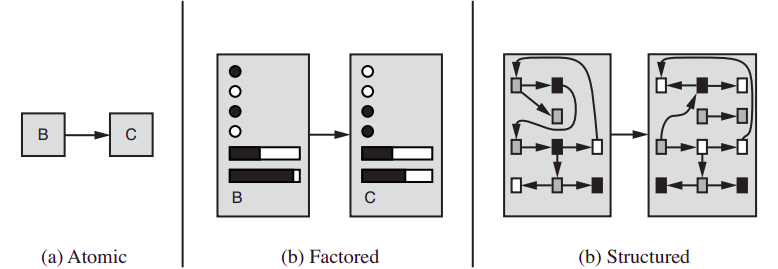
\includegraphics[
        width=\linewidth,
        height=6cm,
        keepaspectratio,
    ]{images/artificial-intelligence/ai-agents/state-representations.png}
    \caption*{
    Three ways to represent states and the transitions between them.
    \\
    \textbf{(a)} Atomic representation: a state (such as B or C) is a black box with no internal structure;  
    \hfill \cite{ai/book/Artificial-Intelligence-A-Modern-Approach/Russell-Norvig}
    \\
    \textbf{(b)} Factored representation: a state consists of a vector of attribute values; values can be Boolean, realvalued, or one of a fixed set of symbols.
    \hfill \cite{ai/book/Artificial-Intelligence-A-Modern-Approach/Russell-Norvig}
    \\
    \textbf{(c)} Structured representation: a state includes objects, each of which may have attributes of its own as well as relationships to other objects.
    \hfill \cite{ai/book/Artificial-Intelligence-A-Modern-Approach/Russell-Norvig}
}
\end{figure}



\begin{enumerate}[itemsep=0.2cm]
    \item Roughly speaking, a more expressive representation can capture, at least as concisely, everything a less expressive one can capture, plus some more. 
    \hfill \cite{ai/book/Artificial-Intelligence-A-Modern-Approach/Russell-Norvig}

    \item Often, the more expressive language is much more concise; for example, the rules of chess can be written in a page or two of a structured-representation language such as first-order logic but require thousands of pages when written in a factored-representation language such as propositional logic.
    \hfill \cite{ai/book/Artificial-Intelligence-A-Modern-Approach/Russell-Norvig}

    \item reasoning and learning become more complex as the expressive power of the representation increases.
    \hfill \cite{ai/book/Artificial-Intelligence-A-Modern-Approach/Russell-Norvig}

    \item To gain the benefits of expressive representations while avoiding their drawbacks, intelligent systems for the real world may need to operate at all points along the axis simultaneously.
    \hfill \cite{ai/book/Artificial-Intelligence-A-Modern-Approach/Russell-Norvig}
\end{enumerate}






\subsection{Atomic representation}

\begin{enumerate}[itemsep=0.2cm]
    \item each state of the world is indivisible - it has no internal structure. 
    \hfill \cite{ai/book/Artificial-Intelligence-A-Modern-Approach/Russell-Norvig}

    \item two different atomic states have nothing in common—they are just different black boxes
    \hfill \cite{ai/book/Artificial-Intelligence-A-Modern-Approach/Russell-Norvig}

    \item Algorithms/ areas that work with atomic representations - or, at least, they treat representations as if they were atomic:
    \begin{enumerate}
        \item Search and game-playing
        \hfill \cite{ai/book/Artificial-Intelligence-A-Modern-Approach/Russell-Norvig}

        \item Hidden Markov models
        \hfill \cite{ai/book/Artificial-Intelligence-A-Modern-Approach/Russell-Norvig}

        \item Markov decision processes
        \hfill \cite{ai/book/Artificial-Intelligence-A-Modern-Approach/Russell-Norvig}
    \end{enumerate}
\end{enumerate}



\subsection{Factored representation}

\begin{enumerate}[itemsep=0.2cm]
    \item A factored representation splits up each state into a fixed set of \textbf{variables} or \textbf{attributes}, each of which can have a \textbf{value}.
    \hfill \cite{ai/book/Artificial-Intelligence-A-Modern-Approach/Russell-Norvig}

    \item two different factored states can \textbf{share} some attributes (such as being at some particular GPS location) and not others (such as having lots of gas or having no gas)
    \\
    this makes it much easier to work out how to turn one state into another
    \hfill \cite{ai/book/Artificial-Intelligence-A-Modern-Approach/Russell-Norvig}

    \item With factored representations, we can also represent uncertainty - for example, ignorance about the amount of gas in the tank can be represented by leaving that attribute blank.
    \hfill \cite{ai/book/Artificial-Intelligence-A-Modern-Approach/Russell-Norvig}

    \item Algorithms/ areas based on factored representations:
    \begin{enumerate}
        \item constraint satisfaction algorithms
        \hfill \cite{ai/book/Artificial-Intelligence-A-Modern-Approach/Russell-Norvig}

        \item propositional logic
        \hfill \cite{ai/book/Artificial-Intelligence-A-Modern-Approach/Russell-Norvig}

        \item planning
        \hfill \cite{ai/book/Artificial-Intelligence-A-Modern-Approach/Russell-Norvig}

        \item Bayesian networks
        \hfill \cite{ai/book/Artificial-Intelligence-A-Modern-Approach/Russell-Norvig}

    \end{enumerate}
\end{enumerate}








\subsection{Structured representation}


\begin{enumerate}[itemsep=0.2cm]
    \item the world as having things in it that are related to each other, not just variables with values.
    \hfill \cite{ai/book/Artificial-Intelligence-A-Modern-Approach/Russell-Norvig}

    \item almost everything that humans express in natural language concerns objects and their relationships
    \hfill \cite{ai/book/Artificial-Intelligence-A-Modern-Approach/Russell-Norvig}

    \item Algorithms/ areas based on factored representations:
    \begin{enumerate}
        \item relational databases
        \hfill \cite{ai/book/Artificial-Intelligence-A-Modern-Approach/Russell-Norvig}

        \item first-order logic
        \hfill \cite{ai/book/Artificial-Intelligence-A-Modern-Approach/Russell-Norvig}

        \item first-order probability models 
        \hfill \cite{ai/book/Artificial-Intelligence-A-Modern-Approach/Russell-Norvig}

        \item knowledge-based learning
        \hfill \cite{ai/book/Artificial-Intelligence-A-Modern-Approach/Russell-Norvig}

        \item natural language understanding
        \hfill \cite{ai/book/Artificial-Intelligence-A-Modern-Approach/Russell-Norvig}
    \end{enumerate}
\end{enumerate}


